\section{Decentralized search for \\ shortest path approximation}
\label{searching}

In this section, we are going to discuss how to perform decentralized searches based on the index structures to achieve a higher accuracy. We will also discuss how to optimize and control the search space of decentralized search to maintain low online search overheads.

%\subsection{Source of error for index-only approximation}
%
%\begin{figure}[t]
    %\centering
    %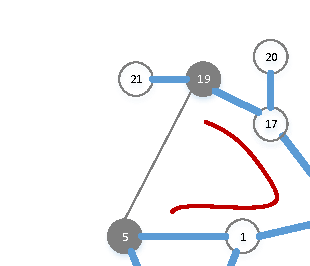
\includegraphics[width=\linewidth]{../figures/new_illustrate/sc_illustrate.pdf}
    %\caption{Edges that do not exist in index cannot be explored while estimating shortest paths solely from labels of source and target vertices. Bold lines represent edges in index.}
    %\label{fig:sc_illustrate}
%\end{figure}
%
%Landmark based algorithms only encode a small portion of edges into the index. Due to that approximated paths only contains edges existing in the index, other edges become the source of approximation errors. For example in Fig. \ref{fig:sc_illustrate}, assuming vertex $0$ is the landmark, bold lines represent edges that have been encoded in the index. Although vertex $4$ and $9$ are adjacent in the underlying graph, the edge $(4,9)$ does not exist in the index. So the path estimated solely by the index $(4, 2, 0, 3, 6, 9)$ will not reflect the true distance of vertex $4$ and $9$. Same problem happens with vertex $5$ and $19$. Even vertices that are not directly connected with these edges may also be effected. For example, from vertex $6$ to $18$, shortest path $(6, 3, 12, 7, 18)$ cannot being extracted directly from the index due to both $(3, 12)$ and $(12, 7)$ are not in the index. Even though we are dealing with sparse graphs, number of edges that have been encoded in index for each landmark is less than the number of vertices, and number of vertices is usually much less than total number of edges. Thus a lot of edges are not encoded in the index. Simply increasing the number of landmarks will encode more edges into the index, which will lead to more accurate results, but also bringing more overheads at same time.

\subsection{Index guided decentralized search}

\begin{figure}[t]
    \centering
    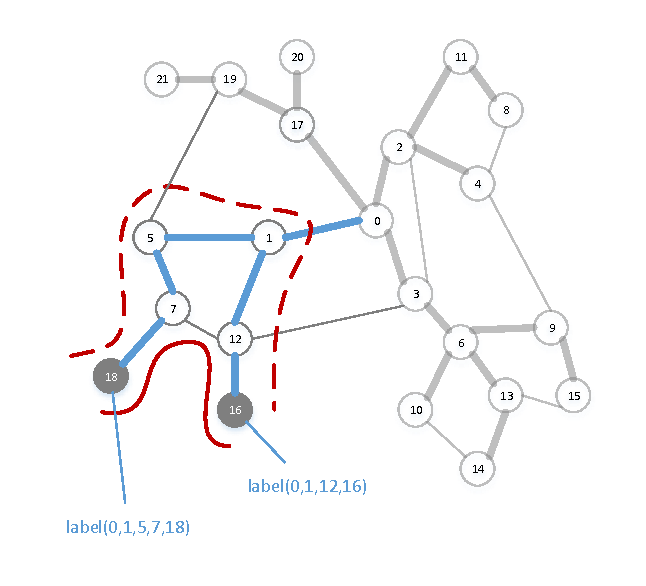
\includegraphics[width=\linewidth]{../figures/new_illustrate/basic_dec.pdf}
    \caption{Decentralized search finds edges that are invisible to labels of the source and target vertices. The dashed curved line shows the path found by LCA distance. The solid curved line shows the path found by the decentralized search.}
    \label{fig:basic_dec}
\end{figure}

By indexing the shortest paths from each landmark in the label of each vertex, we are able to answer both distance and path queries by simple LCA computations with labels of source and target vertices. However, paths returned by LCA computations only contain edges that already exist in the index structure. Observe that, on the other hand, only relatively a small part of the network, i.e., the edges along the shortest path tree, has been indexed. Therefore, such computations may not lead to a high accuracy. For example, in Fig. \ref{fig:basic_dec}, using LCA distances to estimate the shortest path from $18$ to $16$ will return an approximated path $p = (18, 7, 5, 1, 12, 16)$, as represented by the dashed curved line. Note that there is an edge $(7,12)$ that has not been indexed. Therefore, the path $p = (18,7,12,16)$ cannot be found by computing LCA distance directly from labels of vertex $18$ and $16$.

To overcome such difficulties, we use a decentralized search in our design, which, at each step, will examine all the neighbors of current visited vertex and select one that is closest to the target. The search will continue this procedure at each step until it reaches the target vertex. In our case, the distance to the target is estimated by the LCA distance. By calculating the LCA distance to the target from each neighbor, the search can explore edges that do not exist in the labels of source and target vertices. For example, if we use decentralized search in Fig. \ref{fig:basic_dec} to estimate shortest path from $18$ to $16$, when examining neighbors of vertex $7$, vertex $12$ with a LCA distance of $1$ to the target will be selected for next step instead of vertex $5$ with a LCA distance of $3$. In this way, a shorter path can be found by decentralized search through examining edge $(7,12)$ which is not indexed in the labels of source and target vertex.

%Similar to A* search, decentralized search need information on how far each neighbor to the target to determine which vertex to pick as next hop for each step. The difference of decentralized search and A* search is that it makes the decision based solely on local information. By local we mean at each step, decentralized search will only examine the neighbors of currently visited vertex. So all the vertices visited by decentralized search will be a part of the estimated path.

\begin{figure}[t]
    \centering
    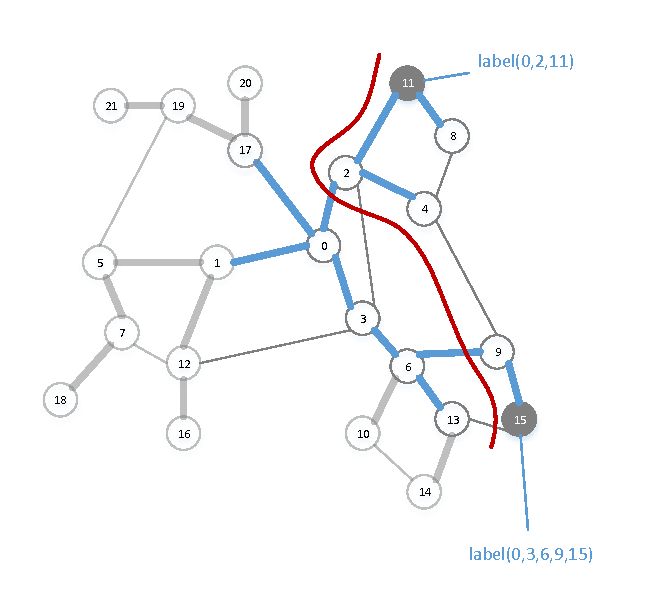
\includegraphics[width=\linewidth]{../figures/new_illustrate/dec_common.pdf}
    \caption{Decentralized search explores the edges that are not directly connected to the indexed shortest path. Edge $(4, 9)$ cannot be found by solely searching circles in the path by LCA distance.}
    \label{fig:dec_common}
\end{figure}

Next, observe that the edge $(7,12)$ shown in Fig. \ref{fig:basic_dec} can also be found by searching if there is any edge existing between any pair of vertices on path returned by LCA computation, so that we can avoid traversing neighbors of any vertex. But this could only find edges that have both ends in the labels of the source and target vertex, which is a very small subset of all the edges. Rather than constraining the search space in this way, decentralized search examines all edges adjacent to current visited vertex, which is a more reasonable and larger subset of edges to examine. For example in Fig. \ref{fig:dec_common} from $15$ to $11$, instead of finding a edge with both ends in labels of vertex $15$: $(0, 3, 6, 9, 15)$ and labels of $11$: $(0, 2, 11)$, decentralized search can find a edge with only one end in label vertex $15$ which has a smaller estimated distance to the target $11$. So that the path denoted by solid curved line can be found. Note that if decentralized search not only examines the edges that adjacent to current visited vertex, but also examines edges that are more than one hop away, shorter paths may be found. But due to the huge number of such edges, they have a relatively low possibility leading to a shorter path on average. Examining them may result in too much overhead. 

\subsection{Early termination}

An important question is that when performing decentralized search based on LCA distances, will the search eventually terminate? The answer is that as long as the source vertex $s$ and target vertex $t$ are reachable from each other, which in our case means that $s$ and $t$ have common landmarks, decentralized search will terminate in as much as $2 * max_{u,v}d_G(u,v)$ steps, where $max_{u,v}d_G(u,v)$ is the diameter of the network. Too see this, note that for the LCA distance of arbitrary source and target vertex $s$ and $t$, the following bound holds:

\begin{equation}
\label{equ:term}
\begin{split}
    d_{LCA}(s,t) \leq max_{l \in L}\{d_G(s,c_l(s,t)) + d_G(c_l(s,t),t)\} \\
		\leq max_{u,v}d_G(u,v) + max_{u,v}d_G(u,v)
\end{split}
\end{equation}

And at each step, as long as the current visited vertex is not the target vertex, there will always be a neighbor with a shorter LCA distance than current visited vertex to the target. So the estimated distance at each step will decrease at least by $1$. Therefore, the LCA distance of arbitrary pairs of vertices is bounded by $2 * max_{u,v}d_G(u,v)$ according to equation \ref{equ:term}. Decentralized search for arbitrary pairs of reachable vertices will terminate in as most $2 * max_{u,v}d_G(u,v)$ steps.

However, terminating only when the search reaches the target vertex is actually not an ideal stopping criterion, and will result in unnecessary overheads by examining redundant edges. Since the label of each vertex stores the shortest path of each vertex to each landmark, the shortest path follows the optimal substructure. That is, the path between any two vertices along the shortest path is also the shortest path of them. Considering that the label of each vertex follows the optimal substructure, the search can actually terminate once it reaches any vertex in the label of the target vertex. Because when the search reaching any vertex in the label of the target vertex, the label has already contained the shortest path from that vertex to the target vertex and decentralized search cannot find a path shorter than this one. Thus, the remaining path can be directly calculated from the label. Actually, decentralized search do not have to traverse vertices along the label of target vertices because these vertices have already been traversed by breadth first search for the same goal, which is reaching target vertex $u$, during preprocessing. With this stop criterion, the search space of decentralized search is significantly reduced and the search can terminate much earlier. The search will only visit at most the number of vertices from source vertex to the least common ancestor of source and target vertices. So the decentralized search can terminate in at most $max_{u,v}d_G(u,v)$ steps. We refer to this optimization as early termination.

\subsection{Bi-directional search}

\begin{figure}[t]
    \centering
    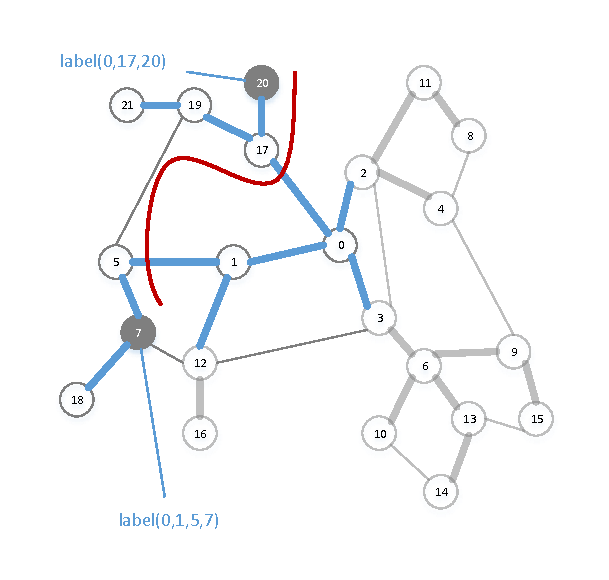
\includegraphics[width=\linewidth]{../figures/new_illustrate/bi_dec.pdf}
    \caption{Bidirectional decentralized search can explore different set of edges which may found path at different length. Searches start at vertex $7$ will lead to a path shorter than starting at $20$ by taking advantage of the edge $(5, 19)$.}
    \label{fig:bi_dec}
\end{figure}

As we have shown above, decentralized search is well suited for exploring the edges that connect currently visited vertex to a vertex that has shorter LCA distance to the target. Intuitively, edges that can lead to a shorter path from target vertex to the source vertex are equally important. By performing the decentralized search twice, one from source to target, and the other from target to source, we can achieve better accuracy by traversing more edges that have equal possibilities leading to shorter paths.

Unlike bidirectional BFS, which is aimed at finding shortest path when two search meet, decentralized search does not guarantee that two searches will meet each other. The only purpose for doing bidirectional decentralized search is to explore more edges that have a high possibility leading to a shorter path. When combining the results of bidirectional decentralized search, one can simply select the path with a shorter length. For example in Fig. \ref{fig:bi_dec}, the search starts from $20$ to $7$ can find a shorter path $p = (20, 17, 19, 5, 7)$ than the search starts at $7$. Due to that $0$ has a smaller LCA distance to $7$ than $19$, the edge $(19, 5)$ cannot be found by the search starts from $20$.

\subsection{Handle ties in decentralized search}

\begin{figure}[t]
    \centering
    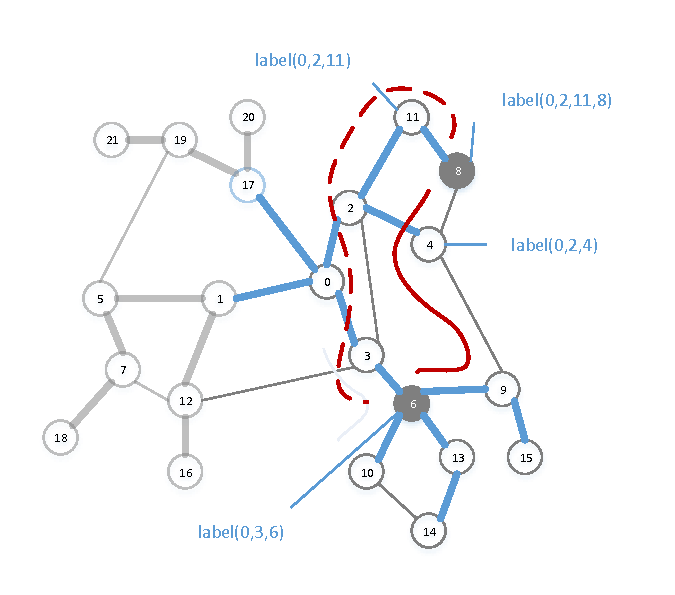
\includegraphics[width=\linewidth]{../figures/new_illustrate/tie.pdf}
    \caption{Tie happens during decentralized search. Although LCA distances are the same, selecting different neighbor will search different part of the graph which may lead to paths at different length.}
    \label{fig:tie}
\end{figure}

Due to the small world property in complex networks, the shortest path tree of the landmark set usually has a limited depth. Furthermore, it is very common that a vertex connects to multiple vertices in a lower level of shortest path tree. So during decentralized search, there is a good chance that the search will encounter a tie at some point, that is, there are several neighbors of current visited vertex that have same shortest LCA distance to the target. For example in Fig. \ref{fig:tie}, to find path from $8$ to $6$, when traversing neighbors of vertex $8$, both vertex $11$ and $4$ have the same LCA distance to vertex $6$, but their actual distances to vertex $6$ are different due to edges currently invisible to the decentralized search. Labels of each neighbor, on the other hand, provide no clue which one can lead to a shorter path.

Since edges at two hops away are invisible to decentralized search, the search has no way to differentiate neighbors when a tie happens. Edges adjacent to these neighbor vertices have the same possibility leading to a shorter path based on information available to the decentralized search. To increase the possibility of finding shorter paths, multiple neighbors with same shortest LCA distance to the target can be selected as candidates for the next hop. In this way, the decentralized search will traverse multiple or even all neighbors with the same shortest LCA distance at the next step. Apparently, doing so will bring extra overheads due to the larger search space. Note that by selecting multiple neighbors, decentralized search can possibly find multiple paths with the same length. This increases the diversity of approximated path of decentralized search, which is required by some applications. 